%% DONE
\id{МРНТИ 20.53.01}{}

\begin{articleheader}
\sectionwithauthors{А. Есенбек, А. Касымова, А. Картбаев}{АНАЛИЗ И КРАТКОСРОЧНОЕ ПРОГНОЗИРОВАНИЕ ЦЕН НА ФОНДОВОМ РЫНКЕ С ПОМОЩЬЮ ВАРИАЦИОННЫХ МОДЕЛЕЙ ВРЕМЕННЫХ РЯДОВ}

{\bfseries А. Есенбек\authorid,
А. Касымова\authorid,
А. Картбаев\textsuperscript{\envelope } \authorid}
\end{articleheader}

\begin{affiliation}
\emph{Казахстанско-Британский технический университет, Алматы, Казахстан}

\raggedright {\bfseries \textsuperscript{\envelope }}{\em Корреспондент-автор: a.kartbaev@kbtu.kz}
\end{affiliation}

Прогнозирование цен на финансовые активы остается жизненно важной
областью финансовой аналитики, что стимулирует постоянные исследования
более эффективных методов прогнозирования. В данном исследовании
рассматривается вопрос о том, можно ли прогнозировать динамику цен на
конкретную акцию на основе движения цен на другие связанные с ней акции.
Наш подход направлен на выявление межфондовых связей и прогнозирование
ценовых тенденций на основе анализа этих связей. Используя машинное
обучение, были выявлены кластеры компаний, демонстрирующих схожие модели
движения цен. Далее использована модель векторной авторегрессии (VAR)
для создания функций импульсного отклика, прогнозирующих потенциальные
колебания цен в последующие дни. Наши эксперименты направлены на
повышение точности и вычислительной эффективности этих прогнозов. Кроме
того, разработана интерактивная панель, которая наглядно отображает
прогнозы изменения цен на акции, позволяя пользователям наблюдать за
ожидаемыми тенденциями цен на акции компаний. Данная работа вносит вклад
в развивающуюся область прогнозного моделирования, улучшая понимание
взаимозависимости между активами и предоставляя доступные прогнозы для
принятия финансовых решений.

{\bfseries Ключевые слова}: машинное обучение, предиктивное моделирование,
прогнозирование цен, нейронные сети, VAR, K-means, Big Data\emph{.}

\begin{articleheader}
{\bfseries УАҚЫТ-ВАРИАЦИЯЛЫ СЕРИЯЛЫҚ МҮЛГІЛЕРДІ ПАЙДАЛАНУ МЕН ҚОР НАРЫҒЫНДАҒЫ БАҒАНЫ ТАЛДАУ ЖӘНЕ ҚЫСҚА МЕРЗІМДІ БОЛЖАУ}

{\bfseries
А. Есенбек,
А. Касымова,
А. Картбаев\textsuperscript{\envelope }}
\end{articleheader}

\begin{affiliation}
\emph{Қазақ-Британ техникалық университеті, Алматы, Қазақстан,}

\emph{e-mail: a.kartbaev@kbtu.kz}
\end{affiliation}

Қаржы активтерінің бағасын болжау қаржылық аналитиканың маңызды саласы
болып қала береді, бұл болжаудың тиімді әдістеріне үздіксіз зерттеулер
жүргізуге түрткі болады. Бұл зерттеу белгілі бір акцияның бағасының
қозғалысын басқа қатысты акциялардың баға қозғалысы негізінде болжауға
болатынын зерттейді. Біздің көзқарасымыз қор аралық байланыстарды
анықтауға және осы байланыстарды талдау негізінде баға үрдістерін
болжауға бағытталған. Нейрондық желілерді пайдалана отырып, біз ұқсас
баға қозғалысы үлгілерін көрсететін компаниялардың кластерлерін
анықтаймыз. Содан кейін біз векторлық авторегрессия (VAR) моделін келесі
күндердегі әлеуетті баға қозғалысын болжайтын импульстік жауап
функцияларын жасау үшін қолданамыз. Біздің эксперименттеріміз осы
болжамдардың дәлдігі мен есептеу тиімділігін арттыруға бағытталған.
Сонымен қатар, біз пайдаланушыларға компания акцияларының бағамындағы
күтілетін үрдістерді көруге мүмкіндік беретін акциялар бағасының
болжамдарын көрнекі түрде көрсететін интерактивті бақылау тақтасын
жасадық. Бұл жұмыс активтер арасындағы өзара тәуелділікті түсінуді
жақсарту және қаржылық шешімдерді қабылдау үшін қолжетімді болжамдарды
қамтамасыз ету арқылы көп акцияларды болжауды модельдеудің пайда болған
саласына ықпал етеді.

{\bfseries Түйін сөздер:} машиналық оқыту, болжамды модельдеу, бағаны
болжау, нейрондық желілер, VAR, K-means, Big Data\emph{.}

\begin{articleheader}
{\bfseries ANALYSIS AND SHORT-TERM PREDICTION OF STOCK MARKET PRICES USING VAR MODELS OF TIME SERIES}

{\bfseries
A. Yessenbek,
A. Kassymova,
A. Kartbayev\textsuperscript{\envelope }}
\end{articleheader}

\begin{affiliation}
\emph{Kazakh-British Technical University, Almaty, Kazakhstan,}

\emph{e-mail: a.kartbaev@kbtu.kz}
\end{affiliation}

Forecasting stock assets prices remains a vital area in financial
analytics, driving ongoing research into more effective predictive
techniques. This study explores whether the price trends of a given
stock can be forecasted based on the price movements of other related
stocks. Our approach seeks to uncover inter-stock relationships and
predict price trends by analyzing these connections. Leveraging neural
networks, we identify clusters of companies exhibiting similar price
movement patterns. Subsequently, we employ a Vector Auto Regression
(VAR) model to generate impulse response functions, projecting potential
price fluctuations over the following days. Our experiments focus on
refining both the accuracy and computational efficiency of these
predictions. Additionally, we developed an interactive dashboard that
visually displays forecasts of stock price changes, enabling users to
observe anticipated trends in companies' stock prices. This work
contributes to the growing field of predictive modeling by enhancing
understanding of interdependencies among stocks and providing accessible
predictive insights for financial decision-making.

{\bfseries Keywords}: machine learning, predictive modeling, stock
forecasting, neural networks, VAR, K-means, Big Data\emph{.}

\begin{multicols}{2}
{\bfseries Введение.} В настоящее время прогнозирование цен на акции и
выявление связей между компаниями - две популярные темы в аналитике
больших данных. Известно, что цены на различные акции коррелируют между
собой; цены на акции иногда движутся вместе. Поэтому вполне естественно
задаться вопросом, можно ли предсказать их цены, используя цены на
другие акции. Цель работы - определить и доказать взаимосвязи между
акциями и спрогнозировать динамику цен на основе изменений цен связанных
с ними финансовых активов. Эта информация может иметь актуальность
исследования для инвесторов, которые хотят принять решение о вложении
средств в определенные виды активов. Понимание взаимосвязей между
акциями может помочь инвесторам обнаружить больше скрытых возможностей,
когда они видят изменения в определенных индексах.

В результате создана модель, которая поможет инвесторам получать
информацию о связях между акциями и прогнозы будущих изменений цен. В
качестве характеристик используются связи в сетях регистраторов фондовых
бирж. Она имеет практическую ценность для организаций, как способ
генерировать оценку из сети и использовать их для предварительного
определения стоимости компании, так и теоретическую ценность для
обучения финансовых моделей методами машинного обучения.

Некоторые другие модели, такие как модель ARIMA {[}1{]} и модель
логистической регрессии {[}2{]}, также используются для этой цели.
Однако эти авторы используют отдельные данные для построения своей
модели и не обращают внимания на связи между компаниями. Кроме того, как
еще одно ограничение данных моделей, они не отбирают признаки перед
прогнозированием новых цен на финансовые активы. Для дальнейшего
развития принято решение использовать VAR-модели {[}3{]}, основанные на
исторических изменениях цен на акции, чтобы получить функции импульсного
отклика, которые предсказывают будущие изменения. Более того, были
использованы группы акций, которые ведут себя одинаково, в качестве
признаков, а не просто используем исторические данные только целевой
акции. Перед прогнозированием цен на акции проведена кластеризация
компаний, чтобы выяснить, какие группы компаний наиболее связаны друг с
другом. Далее эти связанные компаний были использованы в качестве
характеристик VAR-моделей для прогнозирования изменений цен на акции
компаний, выбранных пользователем. Была использована кластеризация
K-means {[}4{]} и ANNOY {[}5{]}, чтобы выяснить, какие группы компаний
связаны между собой, и анализированы преимущества и недостатки наших
методов. Затем результаты кластеризации и модель VAR использованы для
расчета функций импульсного отклика и прогнозирования динамики цен на
основе поиска по сетке для повышения точности и определение времени
работы {[}6{]}.

В последние время, после новаторской работы Симса (1980) по созданию
моделей векторной авторегрессии (VAR) {[}7{]}, эти модели получили
широкое распространение при моделировании взаимосвязей между
экономическими и финансовыми временными рядами и прогнозировании будущих
величин. Поскольку количественные методологии все чаще применяются для
прогнозирования цен на акции, VAR-модели не стали исключением. Во многих
исследованиях VAR-модели использовались для прогнозирования индексов цен
на акции и достигли хороших результатов {[}8 -10{]}. Однако они
моделировали индексы цен акций, а не цены отдельных акций, в то время
как инвесторы часто интересуются будущей доходностью отдельных акций, в
которые они могли бы вложить средства. Ву и Чжоу (2014) рассмотрели
применение моделей VAR для прогнозирования доходности акций, включая
доходность отдельных акций, с относительно теоретической точки зрения и
заложили основу для конкретной, прикладной работы в этой области
{[}11{]}.

В настоящее время в этой области существует не очень большое количество
прикладных работ по данной теме. Например, в работе Лонг (2024)
использовалась модель VAR для прогнозирования дневных максимумов и
минимумов цен на 20 высокоторгуемых акций, и результаты оказались
обнадеживающими: был сделан вывод, что "высокие и низкие цены на акции в
значительной степени предсказуемы {[}12{]}". Однако данные охватывали
только семь лет (2010-2017) и были статичными (не обновлялись
постоянно). Кроме того, рассматривалось лишь небольшое количество акций.

С точки зрения инвесторов, более ценным был бы инструмент
прогнозирования, который можно использовать на большом количестве акций
и который динамически обновляется на основе текущих цен на акции. В
отличие от предыдущих работ, был использован ANNOY для поиска групп
связанных акций, а затем рассчитана VAR-модель под каждую группу. Кроме
того, в предыдущих работах по VAR обычно рассматривалось лишь небольшое
количество акций, в данной работе были включены более 2500 акций.
Поэтому использован динамический подход на основе больших данных для
прогнозирования на основе ежедневно обновляемых цен на акции. Наши
VAR-модели ежедневно обновлялимсь с использованием самых свежих данных о
ценах на акции.Мы полагаем, что такие модели ранее не использовались с
такой степенью широты и глубины для анализа определенных групп активов.

{\bfseries Материалы и методы.} \emph{Данные.} В начале исследования было
собрано данные о более чем 2800 компаниях, входящих в NASDAQ с платформы
Kaggle начиная с момента выхода на биржу, в зависимости от доступности
информации в наиболее полном объеме. Для каждой акции и для каждого дня
были включены данные о низкой цене, цене открытия, объеме, высокой цене,
цене закрытия и скорректированной цене закрытия. Причем размер этих
данных составил около 19 ГБ, а формат включает, в основном, \emph{json}
и \emph{csv}.

Кроме того, наши данные обновлялись с помощью модуля yfinance в Python,
который загружает цены на акций через Yahoo Finance.

В результате модель обновляла около 5-6 МБ дополнительных данных каждый
будний день. Эти новые данные обрабатываются в формате процентных
изменений и затем используются для обновления существующего набора
данных, что гарантирует, что модели всегда будут соответствовать самой
актуальной информации.

Эти данные были очищены с помощью библиотеки Pandas. Были отброшены
акции, по которым имеется слишком мало данных, то есть если они были
опубликованы менее четырех лет назад. Это связано с тем, что по таким
акциям у нас нет достаточной информации для точной оценки их взаимосвязи
с другими акциями и прогнозирования их будущих ценовых тенденций. Также
были исключены акции, которые больше не торгуются на рынке. В результате
всего насчитано 2511 акций. Затем данные были обработаны в формате,
удобном для наших моделей. Далее данные переведены в формат процентных
изменений. Также были добавлены к данным аддитивная обратная величина
для каждой акции, чтобы выявить акции которые отрицательно связаны с
другими акциями.
\end{multicols}

\begin{figure}[H]
	\centering
	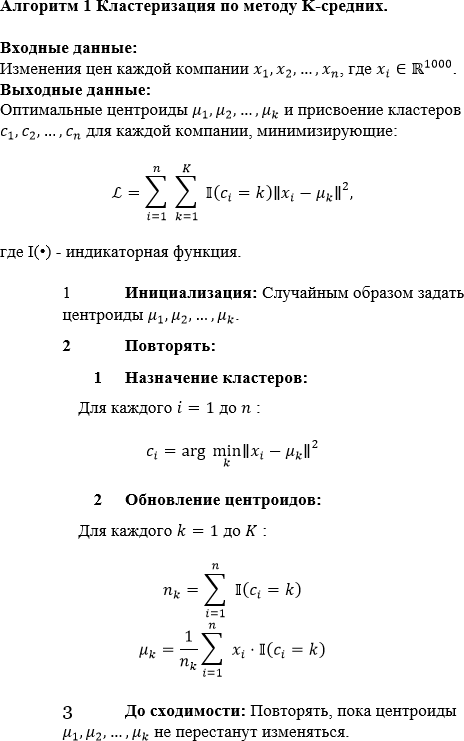
\includegraphics[width=0.5\textwidth]{media/ict2/image3}
	\caption*{Рис. 1 - Алгоритм 1. Кластеризация по методу K-средних}
\end{figure}

\begin{multicols}{2}
\emph{Кластеризация по методу К-средних}. Было изучен метод
кластеризации K-means clustering, где использовались К-средние для
кластеризации компаний на основе изменений их биржевых цен. Поскольку
целью кластеризации является получение связей между компаниями, группы,
имеющие только одну компанию, не могут дать нам никакой информации.
Поэтому алгоритм использован следующим образом, как на рисунке 1.

Для работы модели VAR необходимы кластеры акций. Естественно рассмотреть
модели обучения без контроля, такие как k-means. Однако для того, чтобы
неконтролируемое обучение давало хорошее представление данных, то есть
кластеры с одинаковым размером, данные должны быть линейно разделимыми
по своей сути. В связи с тем, что размер кластеров в данных по акциям
сильно разбалансирован, был использован алгоритм ближайших соседей.

Был выбран ANNOY из-за высокой скорости и универсальности. Эта вариация
метода широко используется в производстве функций поиска и ранжирования
технологических компаний, таких как Netflix. Это библиотека для python,
которая является самым быстрым способом ее практической реализации, где
она случайным образом разрезает данные на небольшие фрагменты, пока все
фрагменты не станут меньше n.

Затем он строит лес бинарных деревьев, в котором каждая режущая
гиперплоскость является внутренним узлом, а каждый осколок - внешним
узлом. Для поиска цели перебираются деревья от корня до соответствующего
внешнего узла, содержащего цель и ближайшие осколки, если в узле меньше
точек, чем нам нужно, как показано на рисунке 2. Результат поиска по
всем деревьям используется для получения рейтинга сходства.
\end{multicols}

\begin{figure}[H]
	\centering
	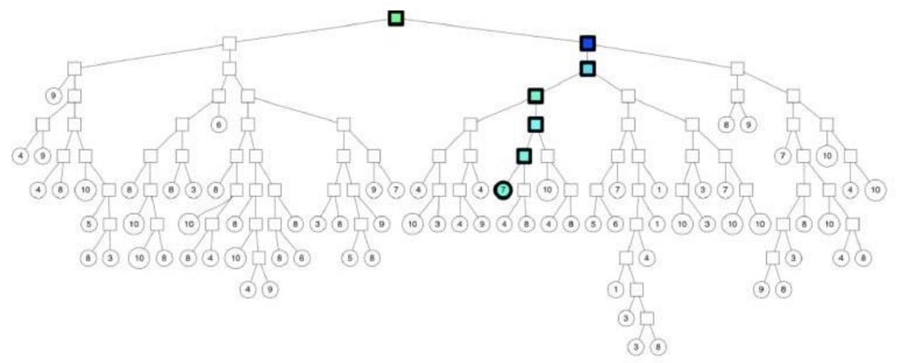
\includegraphics[width=\textwidth]{media/ict2/image4}
	\caption*{Рис. 2 - Бинарное дерево ANNOY}
\end{figure}

\begin{multicols}{2}
После очистки фактические цены были преобразованы в процентные
изменения. В качестве признаков были взяты цены закрытия за последние
1000 дней. Чтобы понять отрицательную корреляцию между акциями, также
добавлен к данным аддитивный обратный вектор. Затем было построено
бинарное дерево ANNOY с векторным представлением каждой акции, используя
евклидово расстояние как метрику сходства. Модель выводит 10 наиболее
похожих акций и соответствующее сходство для каждого поиска. Названия
акций с меткой "inversed" указывают на сильную отрицательную корреляцию.
В нашей системе был построен ANNOY, которая принимает на вход коды акций
и ищет по ним соответствующий вектор. Выходные данные также
преобразуются в названия акций из вектора.

\emph{Модель VAR.} Сразу после получения группы акций с помощью ANNOY,
далее рассмотрена модель векторной авторегрессии (VAR) для акций этой
группы. Модели VAR используются для моделирования отношений между
несколькими временными рядами. Поскольку исторические цены каждой акции
представляют собой временной ряд, VAR-модели хорошо подходят для
моделирования взаимосвязи между ценами на акции. Она состоит из системы
линейных уравнений, где каждый ряд рассматривается как зависимая
переменная в одном уравнении, а независимыми переменными являются
значения каждого временного ряда в предыдущие периоды. Например, простая
VAR-модель двух временных рядов у 1 и у 2 может быть записана следующим
образом:
\end{multicols}

\begin{equation}
\begin{matrix}
y_{1t} = \beta_{10} + \beta_{11}y_{1t - 1} + \alpha_{11}y_{2t - 1} + u_{1t} \\
y_{2t} = \beta_{20} + \beta_{21}y_{2t - 1} + \alpha_{21}y_{1t - 1} + u_{2t}
\end{matrix}
\end{equation}

далее можно записать в виде:

\begin{equation}
\left( \begin{array}{r}
y_{1t} \\
y_{2t}
\end{array} \right) = \left( \begin{array}{r}
\beta_{10} \\
\beta_{20}
\end{array} \right) + \begin{pmatrix}
\beta_{11} & \alpha_{11} \\
\alpha_{21} & \beta_{21}
\end{pmatrix}\left( \begin{array}{r}
y_{1t - 1} \\
y_{2t - 1}
\end{array} \right) + \left( \begin{array}{r}
u_{1t} \\
u_{2t}
\end{array} \right)
\end{equation}

\begin{multicols}{2}
где \(y_{1t}\) и \(y_{2t}\) представляют собой значения у 1 и у 2 в
момент времени \(t,y_{1t - 1}\) и \(y_{2t - 1}\) представляют значения у
1 и у 2 в момент времени \(t - 1\) n \(\beta s\) и \(\alpha s\)
коэффициенты, подлежащие оценке.

Было решено использовать VAR-модели, поскольку они имеют несколько
важных преимуществ при моделировании отношений между акциями. Во-первых,
в VAR-модели каждая переменная рассматривается как зависимая. Это
позволяет полностью отразить динамические отношения между акциями;
например, если цена акции X изменится, это может привести к изменению
цены акции Y, которая затем может привести к другому изменению цены
акции X. Модели VAR очень хорошо отражают этот тип сложной зависимости,
в то время как другие регрессионные модели, такие как линейная
регрессия, отражают зависимость только в одном направлении, поскольку в
них некоторые акции рассматриваются как независимые переменные.

Таким образом, по сравнению с другими регрессионными моделями,
VAR-модели наиболее подходят для полного и точного ответа на наш вопрос.
Еще одно преимущество VAR-моделей заключается в том, что их легко
оценивать, оценка производится с помощью обыкновенных наименьших
квадратов для каждого уравнения. Кроме того, VAR-модели обладают
хорошими возможностями предсказывать цены на много дней вперед, а не
только на следующий день. Это важно, поскольку инвесторов часто
интересует, как изменятся цены на акции в ближайшие несколько недель, а
не только завтра. Наконец, четкая структура VAR-моделей позволяет легко
интерпретировать результаты и прогнозы, что помогает инвесторам
воплотить полученные результаты в реальные решения.

При каждом выполнении поиска акций в модели происходит оценка VAR-модель
на группе из 10 акций, найденных с помощью ANNOY, поэтому VAR-модель
состоит из 10 уравнений. Независимыми переменными являются цены каждой
из 10 акций на день раньше (день \(t - 1\) ). Эта VAR-модель может быть
записана как:
\end{multicols}

\begin{equation}
\begin{matrix}
y_{1,t} = b_{1,0} + b_{1,1}y_{1,t - 1} + b_{1,2}y_{2,t - 1} + \cdots + b_{1,10}y_{10,t - 1} + e_{1,t} \\
y_{2,t} = b_{2,0} + b_{2,1}y_{1,t - 1} + b_{2,2}y_{2,t - 1} + \cdots + b_{2,10}y_{10,t - 1} + e_{2,t} \\
y_{10,t} = b_{10,0} + b_{10,1}y_{1,t - 1} + b_{10,2}y_{2,t - 1} + \cdots + b_{10,10}y_{10,t - 1} + e_{10,t}
\end{matrix}
\end{equation}

\begin{multicols}{2}
где \(y_{i,t}\) цена акции і в день t , а все b - коэффициенты,
подлежащие оценке. Эквивалентно, в векторной форме, эта модель VAR имеет
вид:

\begin{equation}
Y_{t} = B_{0} + B_{1} \ast Y_{t - 1} + e_{t}
\end{equation}

где \(Y_{t}\) вектор 10 х 1 цен на акции в день t и \(B_{0}\) и
\(B_{1}\) матрицы коэффициентов 10 x 1 и 10х10, подлежащих оценке.
Модель VAR оценивается с помощью библиотеки statsmodels в Python. После
оценки модели вычислены функции импульсного отклика, которые
предсказывают, как изменение цены данной акции в настоящий день повлияет
на цены других акций в последующие дни.

Несмотря на множество очевидных преимуществ, которыми обладают
VAR-модели, у них есть и недостаток. Было запланировано применение
VAR-модели к группам связанных акций. Поскольку количество
коэффициентов, которые необходимо оценить в модели, быстро растет с
увеличением числа переменных (например, если переменных n, то существует
\(n^{2}\) коэффициентов, каждый из которых все сложнее вычислить при
увеличении n), не представляется возможным за разумное время построить
VAR-модели для групп из более чем 100 акций. Особенно учитывая, что
модели оцениваются в реальном времени, когда пользователи ищут
определенную акцию в приложении, малое время работы очень важно. Однако,
когда была предпринята попытка создать группы связанных акций с помощью
кластеризации K-means, некоторые группы оказались слишком большими (
\(100\) акции), независимо от того, какое количество кластеров были
использованы. Поэтому были рассмотрены несколько других методов поиска
групп связанных акций, таких как ЕМ-алгоритмы и KNN, и в итоге решили
создать группы с помощью приближенных ближайших соседей, благодаря
существованию библиотеки ANNOY на языке python с быстрым временем
выполнения.

{\bfseries Результаты и обсуждение.} Задача заключалась в предсказании цен
на акции на ближайшие несколько дней с использованием моделей VAR. Для
оценки точности прогнозов случайным образом были выбраны 50 акций и 20
дней в качестве тестовых примеров. Затем для каждого из тестовых
примеров был осуществлен поиск группы связанных акций с помощью ANNOY,
после чего построили VAR-модель для прогнозирования цен на акции на
следующие несколько дней. Прогнозы сравнивались с фактическими ценами в
эти дни, чтобы вычислить среднюю абсолютную ошибку прогнозов. Также были
рассчитаны средняя погрешность прогнозов, т. е. то, насколько прогнозы в
среднем выше или ниже фактических цен, более полные данные приведены
ниже в Таблице 1.
\end{multicols}

\begin{table}[H]
\caption*{Таблица 1 - Измерения точности работы модели}
\centering
\begin{tblr}{
  cells = {c},
  hlines,
  vlines,
}
История\_Дней & Прогноз\_Дней & Кол\_Акций & Сред.кв. ошибка \\
900           & 5             & 10         & 0.009192        \\
900           & 5             & 9          & 0.009298        \\
900           & 10            & 7          & 0.009582        \\
900           & 3             & 7          & 0.010905        \\
700           & 10            & 10         & 0.086412        \\
700           & 10            & 7          & 0.086470        \\
700           & 3             & 7          & 0.011312        \\
900           & 10            & 9          & 0.011659        \\
900           & 10            & 5          & 0.088065        \\
300           & 3             & 10         & 0.012224        \\
300           & 10            & 9          & 0.087300        
\end{tblr}
\end{table}

\begin{multicols}{2}
Чтобы минимизировать среднюю абсолютную ошибку, был проведен сеточный
поиск для оптимизации гиперпараметров модели, а именно продолжительности
обучения, продолжительности прогнозирования и количества акций в группе.
То есть для каждого тестового случая было использовано разное количество
связанных акций и разное количество дней обучения, чтобы предсказать
цены в разное количество будущих дней. Для этого был поиск с длиной
обучения {[}1200, 900, 700, 500, 300, 150, 30{]}, длительность
прогнозирования {[}3, 5, 15, 30{]} и размер кластера {[}5, 12, 15{]}.
Это показало, что оптимальными гиперпараметрами являются 600 дней
обучения, 5-7 дней прогнозирования и до 10 акций на группу. Это
позволило достичь средней абсолютной ошибки 0.089\%, как указано в
Таблице 1. Рассматривая каждый тестовый случай в отдельности, было
обнаружено, что модель с оптимальными гиперпараметрами достигла
абсолютной ошибки в диапазоне \(0 - 1\text{\%}\) в широком диапазоне
отраслей и во времени. Более того, смещение прогнозов было близким к
нулю (\(\) \(- 0.1\text{\%}\) и \(0.1\text{\%}\)) для всех тестовых
случаев, что говорит о том, что цены акций не переоцененные и не
недооцененные.

Также была оценка времени работы программы для 20 случайно выбранных
акций. Напомним, что всякий раз, когда запрашиваются результаты по
определенной акции, используется ANNOY для поиска группы связанных
акций, а затем подгоняют под эту группу модель, чтобы сгенерировать
функции импульсного отклика, которые предсказывают будущие изменения
цен. Было обнаружено, что общее время работы программы составляет от 1,2
до 1,6 секунды. Таким образом, пользователи приложения могут ожидать
результатов в течение 1,5 секунд после выполнения поиска. Из общего
времени работы построение и запрос ANN-модели занимает до 0,4 секунды, а
оценка модели и вычисление функций импульсного отклика до 0,03 секунды.

Во время выполнения программы каждый день оператор python вызывает
функцию, которая загружает цены на акции с помощью модуля yfinance,
обрабатывает их в нужном нам формате и сохраняет в csv-файл. Когда
пользователь ищет определенную акцию в нашем приложении, вызывается
функция, которая с помощью ANNOY находит 10 наиболее тесно связанных
акций, а затем оценивает модель VAR, используя исторические цены этих 10
акций. Затем рассчитываются функции импульсного отклика для каждой из 10
компаний по сравнению с искомой компанией, и результаты отображаются в
виде таблицы. Кроме того, используется функция импульсного отклика для
выработки инвестиционных рекомендаций. Для каждой из десяти компаний,
если прогнозируемое кумулятивное изменение цены положительно по крайней
мере в 4 из следующих 5 дней, рекомендуется "покупать"; если
прогнозируемое кумулятивное изменение цены отрицательно по крайней мере
в 4 из следующих 5 дней, рекомендуется "продавать"; в противном случае
предлагают "нейтральную" рекомендацию. Эти рекомендации также
отображаются в таблице. Ниже приведен рисунок 3, где показано прогноз
изменения цены акций на следующие пять дней.
\end{multicols}

\begin{figure}[H]
	\centering
	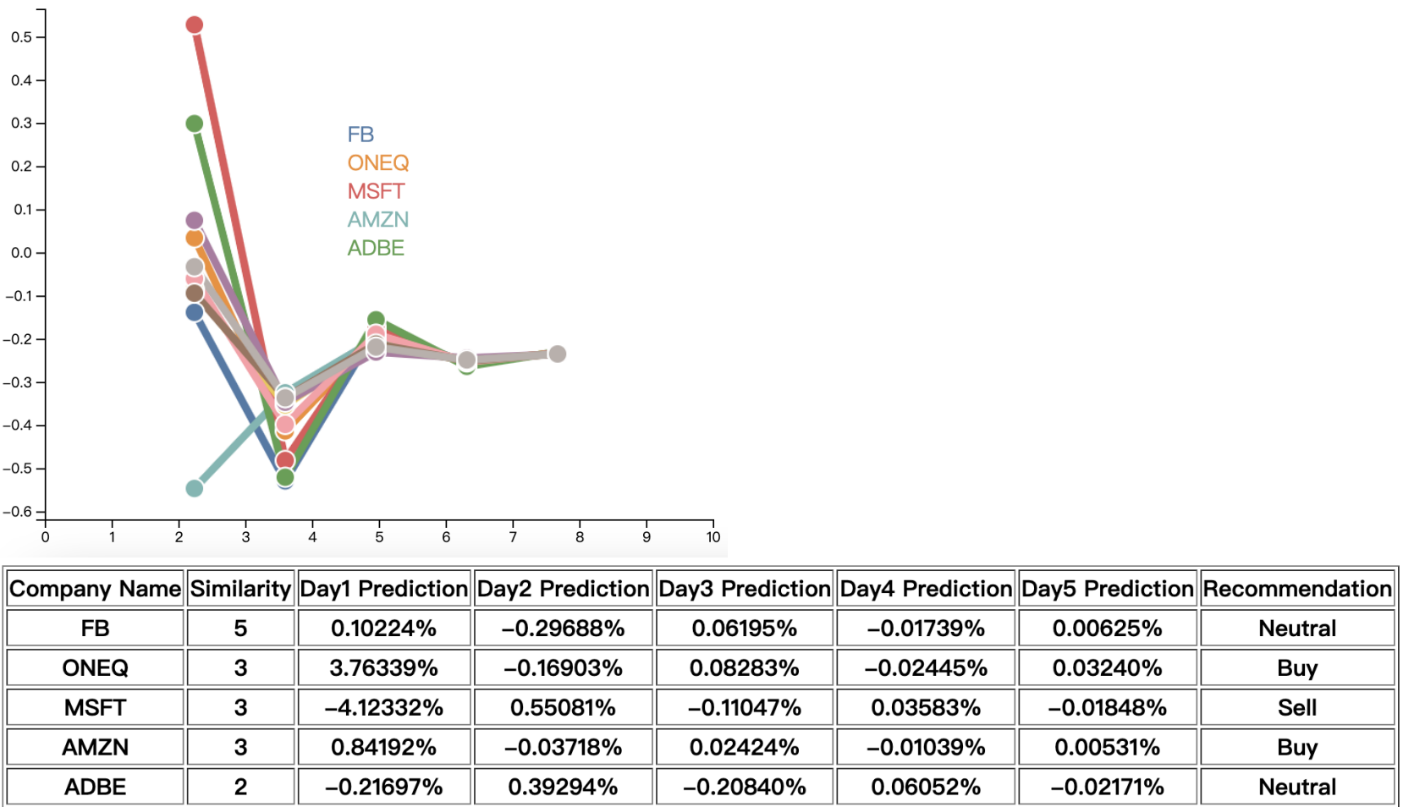
\includegraphics[width=0.85\textwidth]{media/ict2/image5}
	\caption*{Рис. 3 - Прогноз изменения цены акций на следующие пять дней по модели}
\end{figure}

\begin{multicols}{2}
Эти рекомендации рассчитаны помочь пользователям более эффективно
принимать решения на основе полученных прогнозов. После того как
пользователь введет название компании и выберет цель поиска (отклик),
полученные данные будут переданы в бэкенд. Функция get results в view.ру
создаст модель ANNOY и VAR, используя csv-файл в главной директории, и
вернет результаты, которые будут отправлены на фронт-енд для построения
визуализации с помощью функции annoyvar в views.py, где будет отображен
VAR. Во-первых, входные данные, подаваемые в таблицу А, будут отображать
сходство каждой связанной акции с искомой, рекомендуемую операцию и
фактические прогнозируемые процентные изменения в ближайшие 5 дней.

Чтобы улучшить подход, был построен динамический линейный график,
который изначально отображает прогнозы по всем акциям. Поскольку у
каждой компании есть различные связанные акции, и даже эта группа
меняется каждый день, нет возможности просто обучить одну модель и
вызывать ее каждый раз. Поэтому система мгновенно строит отдельную
модель для искомой акции. Преимущество заключается в том, что модель
всегда обновляется и не требует большого пространства для хранения.

{\bfseries Выводы.} В результате была достигнута цель исследования по
прогнозированию трендов цен на акции и отношений между акциями. Теперь
на основе исследований получен инструмент, который может показать
отношения между акциями, а также может предсказывать изменения цен на
акции на следующие семь дней и предоставлять пользователям рекомендации.
В процессе работы над данным проектом были выявлены многие ранее
неизвестные проблемы. Изначально было решено использовать k-means для
кластеризации, но позже обнаружили, что использование k-means метода
приведет к множеству проблем для прогнозирования цены акций в паре с
моделью VAR. Было решено использовать ANNOY для более полного решения
этой проблемы. Когда исследование только началось было неизвестно, как
динамически подключать результаты в модель из различных форматов данных.
Позже было изучено, как другие модели решали эту проблему, и, наконец,
проблема была решена самостоятельно с помощью методов из библиотеки на
языке python. Также изначально не было известно, какой объем данных
использовать для прогнозирования, а также неизвестно, через сколько дней
после прогнозирования результаты будут наиболее точными. Но, для этого
были использованы результаты поиска по сетке, чтобы выбрать параметры с
наименьшей погрешностью.

В результате функции импульсного отклика рассчитываются непосредственно
по коэффициентам модели VAR, с учетом всех разнонаправленных связей
между ценами акций, определяемых каждым уравнением модели. Существует
еще несколько будущих улучшений, которые можно сделать в рамках этой
работы. Во первых, сейчас возможно простое предсказание изменения цен на
акции на ближайшие несколько дней, поскольку результаты прогнозирования
изменений цен на акции сходятся с моделью. Если нужно предсказывать цены
на акции в течение очень долгого времени, то вероятно следует
использовать другие более специализированные методы. Более того, была
достигнута улучшение модели за счет уменьшения ошибок в процессе оценки
изменений трендов.
\end{multicols}

\begin{center}
{\bfseries Литература}
\end{center}

\begin{references}
1. George E.P. Box, Gwilym M. Jenkins, Gregory C. Reinsel and Greta M.
Ljung Time Series Analysis: Forecasting and Control,5th Edition.
-Published by John Wiley and Sons Inc., Hoboken, New Jersey, 2015. --P.
712. ISBN 978-1-118-67502-1

2. David W Hosmer, S. L. Lemeshow Applied Logistic Regression. -John
Wiley \& Sons, New York, 2000. DOI 10.1002/0471722146

3. Agus Suharsono; Auliya Aziza; Wara Pramesti Comparison of vector
autoregressive (VAR) and vector error correction models (VECM) for index
of ASEAN stock price // AIP Conference Proceedings. - 2017. -Vol. 1913.
DOI 10.1063/1.5016666

4. J. MacQueen. Some methods for classification and analysis of
multivariate observations // Berkeley Symp. on Math. Statist. and Prob.
-1967. -Vol. 5.1. -P. 281--297. URL:
\href{http://projecteuclid.org/euclid.bsmsp/1200512992}{http://projecteuclid.org}

5. Erik BernhardssonANNOY: Approximate Nearest Neighbors in C++/Python //
Github pages. -2014. URL: https://github.com/spotify/annoy

6. Bergstra J., Bengio Yo. Random search for hyper-parameter
optimization// Journal of Machine Learning Research. -2012. -Vol. 13.
-P. 281--305. DOI 10.5555/2188385.2188395

7. Christopher A. Sims Macroeconomics and Reality// Econometrica. -1980.
-Vol. 48. -P. 1--48. DOI 10.2307/1912017

8. Helmut Lütkepohl New Introduction to Multiple Time Series Analysis:
textbook. - 2005. ISBN 978-3-540-40172-8

9. Lutz Kilian,, Helmut Lütkepohl Structural Vector Autoregressive
Analysis. -Cambridge University Press, 2017. DOI 10.1017/9781108164818

10. Ruey S. Tsay Analysis of Financial Time Series. -- Wiley, 2010. -720
p. ISBN 9780470414354

11. David R. Rapach, Matthew C. Ringgenberg, , Guofu Zhou Short interest
and aggregate stock returns // Journal of Financial Economics. -2016.
-Vol. 121(1). -P. 46-65. DOI 10.1016/j.jfineco.2016.03.004

12. Wen Long \& Jing Gao \& Kehan Bai \& Zhichen Lu A hybrid model for
stock price prediction based on multi-view heterogeneous data //
Financial Innovation, Springer;Southwestern University of Finance and
Economics. -2024. -Vol. 10(1). --P. 1-50. DOI 10.1186/s40854-023-00519-w
\end{references}

\begin{authorinfo}
\emph{{\bfseries Cведения об авторах}}

Есенбек А.- магистрант, Казахстанско-Британский технический университет,
Алматы, Казахстан, e-mail: \\a\_yessenbek@kbtu.kz;

Касымова F.- магистрант, Казахстанско-Британский технический
университет, Алматы, Казахстан, e-mail: \\a\_kassymova@kbtu.kz;

Картбаев А.-PhD, ассоциированный профессор, Казахстанско-Британский
технический университет, Алматы, Казахстан, e-mail: a.kartbaev@kbtu.kz.

\emph{{\bfseries Information about the authors}}

Yessenbek A.- master student, Kazakh-British Technical University,
Almaty, Kazakhstan, e-mail: a\_yessenbek@kbtu.kz;

Kassymova F.- master student, Kazakh-British Technical University,
Almaty, Kazakhstan, e-mail: a\_kassymova@kbtu.kz;

Kartbayev A. -- PhD, associate professor, Kazakh-British Technical
University, Almaty, Kazakhstan, e-mail: a.kartbaev@kbtu.kz.
\end{authorinfo}
